\documentclass[10pt]{beamer}
\usetheme{Madrid}
\usepackage[spanish]{babel}
\usepackage{graphicx}
\usepackage{tabularx}
\usepackage{booktabs}
\usepackage{enumitem}

\title{Sistema de Reservas de Salas de Estudio UTP}
\subtitle{Avance de Proyecto 1 - Diseño de Productos y Servicios}
\author{Luis Huatay Salcedo \and Cindel Roxell García Chumpitaz \\ Fernando Raúl Díaz Benítez \and Bryan Alexander Quispe Fernandez}
\institute{Universidad Tecnológica del Perú}
\date{19 de abril de 2025}
\logo{
\includegraphics[height=1cm]{assets/logo-utp.png}} % Reemplaza con tu logo

\begin{document}

\begin{frame}
\titlepage
\end{frame}

\section{Introducción}
\begin{frame}{Introducción}
\begin{block}{Contexto}
La UTP necesita optimizar el uso de sus salas de estudio mediante un sistema digital que:
\begin{itemize}
\item Facilite reservas rápidas y sencillas
\item Garantice disponibilidad real de espacios
\item Mejore la experiencia educativa
\end{itemize}
\end{block}

\begin{exampleblock}{Beneficios esperados}
\begin{itemize}
\item Entorno propicio para aprendizaje
\item Colaboración efectiva entre estudiantes
\item Uso eficiente de infraestructura
\end{itemize}
\end{exampleblock}
\end{frame}

\section{Definición del problema}
\begin{frame}{Problema actual}
\begin{columns}
\column{0.5\textwidth}
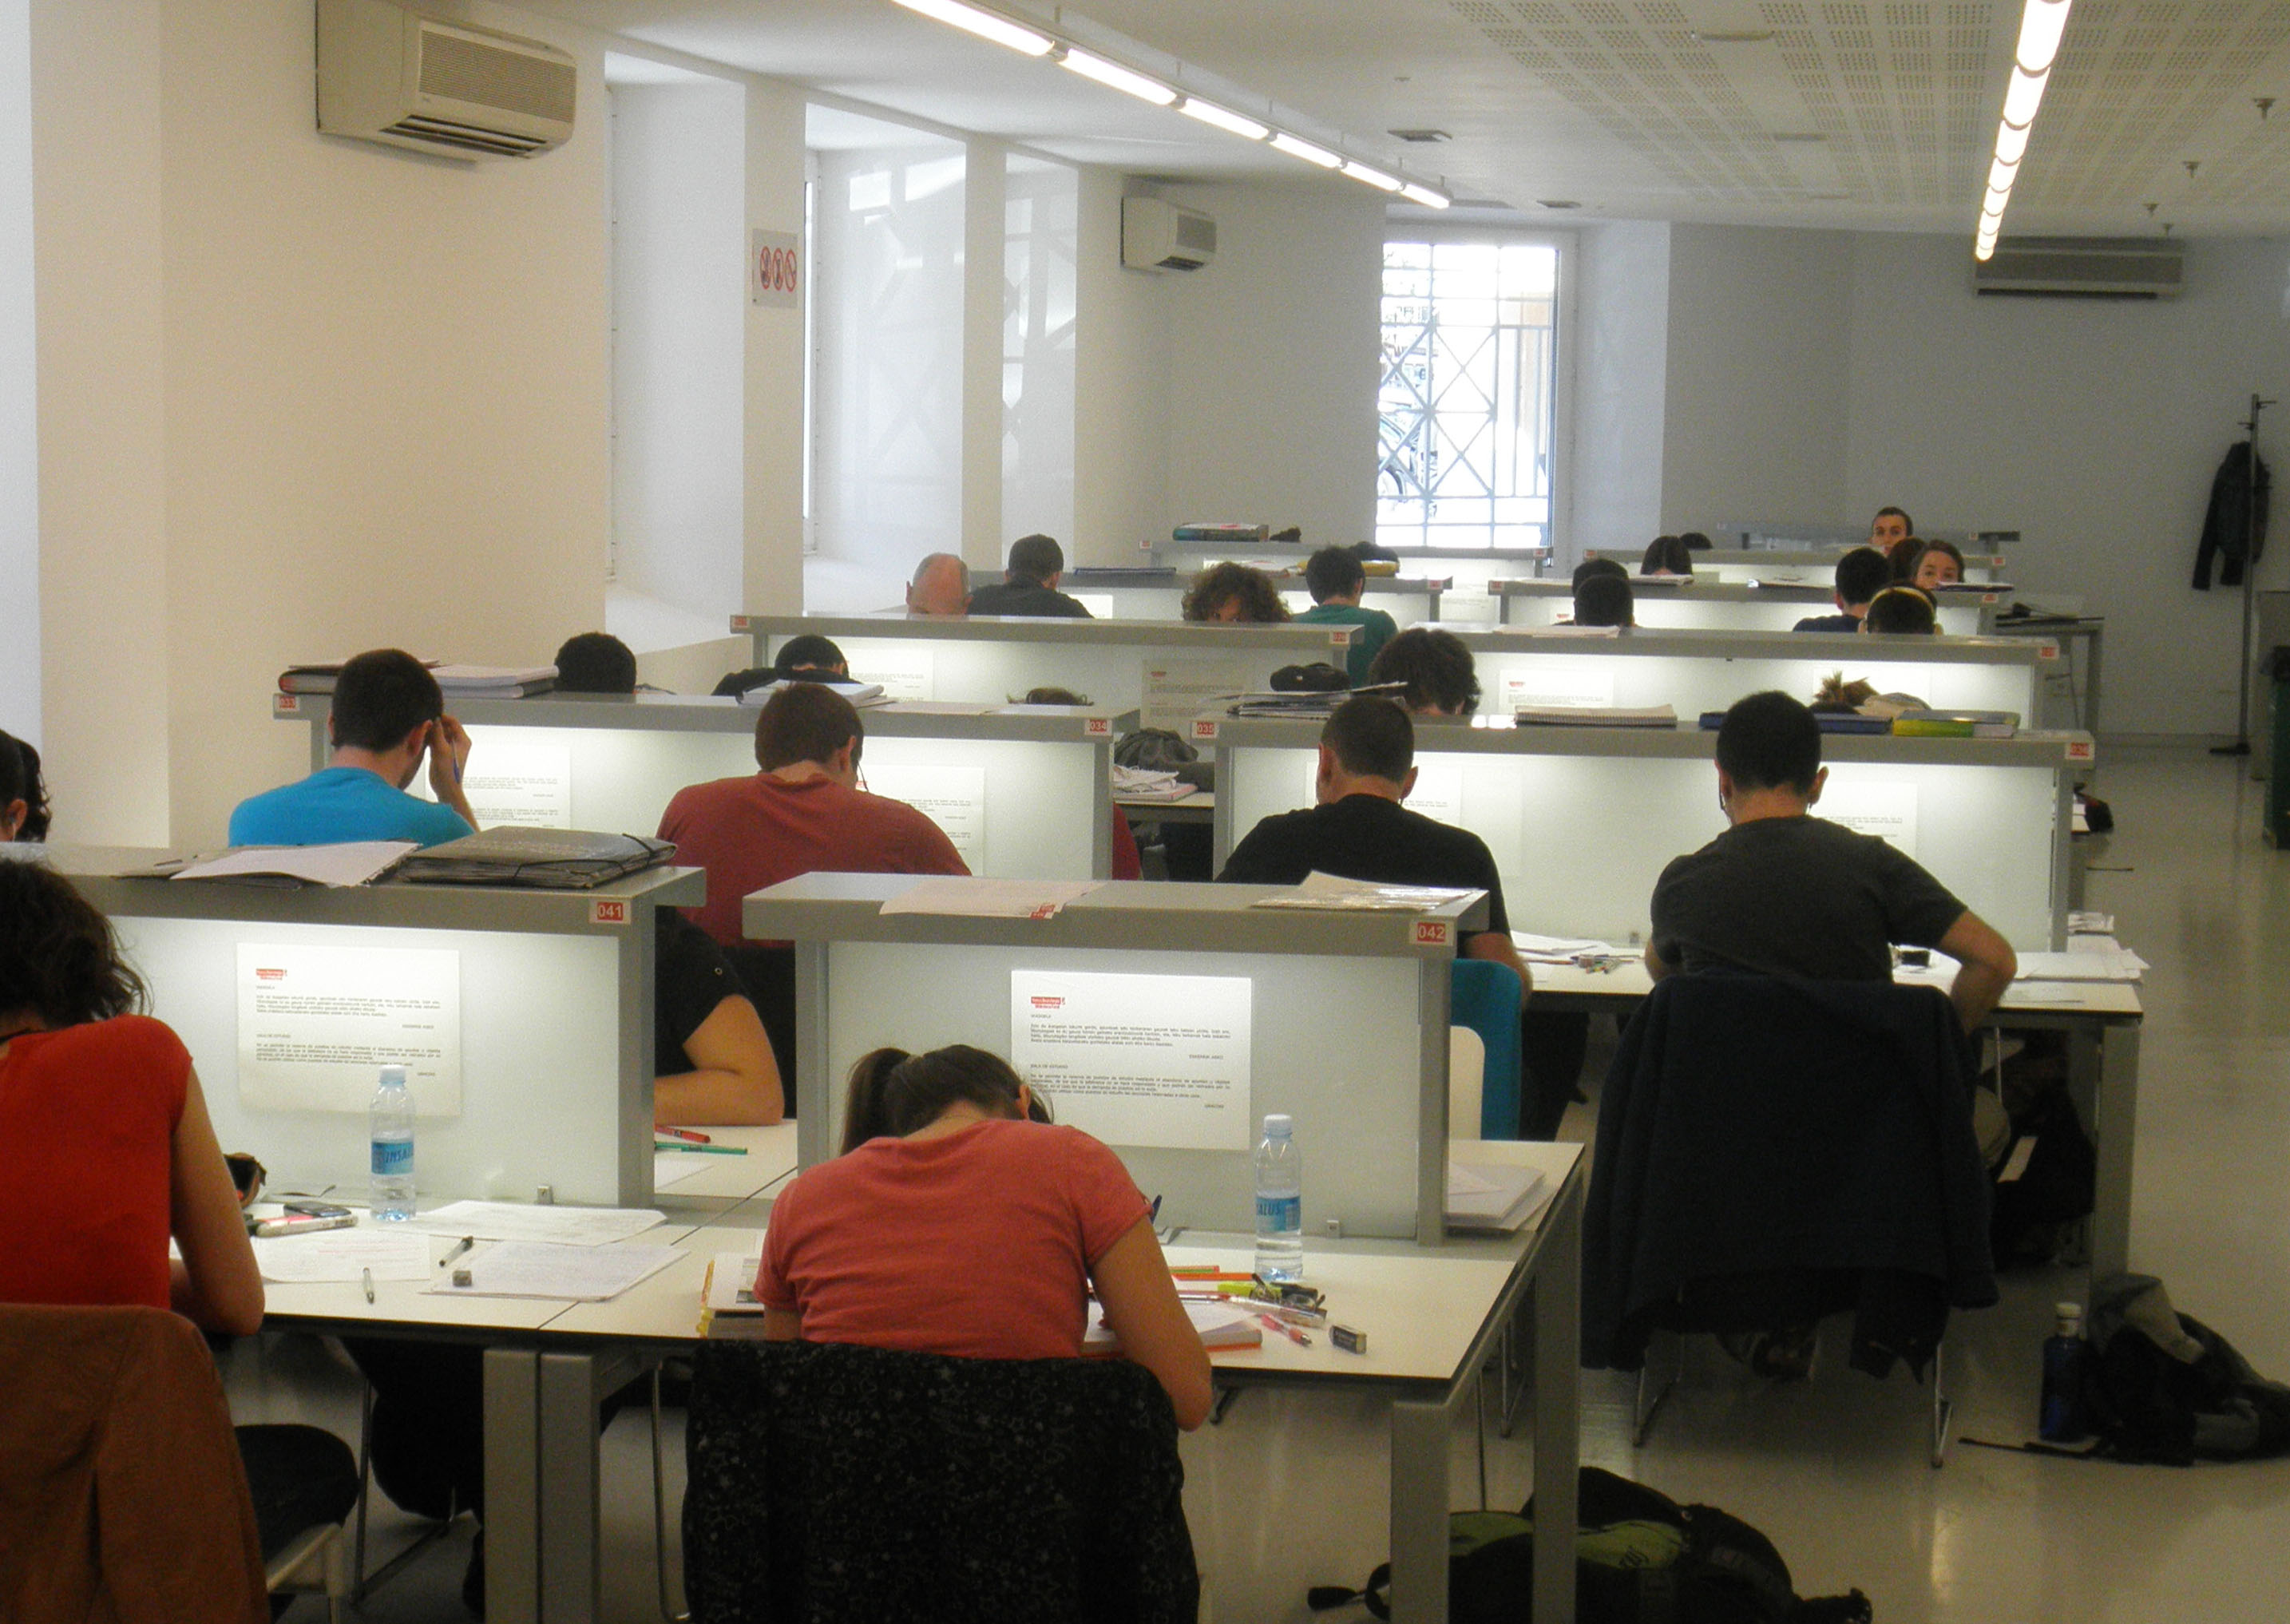
\includegraphics[width=\textwidth]{assets/ocupada.jpg} % Reemplaza con imagen real
\column{0.5\textwidth}
\begin{alertblock}{Principales dificultades}
\begin{itemize}[leftmargin=*]
\item Sistema digital ineficiente
\item Desorganización en reservas
\item Conflictos entre estudiantes
\item Falta de información en tiempo real
\end{itemize}
\end{alertblock}
\end{columns}
\end{frame}

\begin{frame}{Solución propuesta}
\begin{center}
\Large Plataforma web/app que permita:
\end{center}

\begin{itemize}
\item Reservas instantáneas
\item Notificaciones de disponibilidad
\item Gestión inteligente de espacios
\item Liberación automática de salas no utilizadas
\end{itemize}

\begin{center}
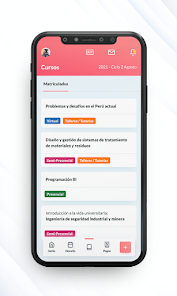
\includegraphics[height=2cm]{assets/app.png} % Reemplaza con mockup
\end{center}
\end{frame}

\section{Investigación de usuarios}
\begin{frame}{Hallazgos clave}
\begin{table}[ht]
\centering
\small
\begin{tabular}{p{0.3\textwidth} p{0.6\textwidth}}
\toprule
\textbf{Aspecto} & \textbf{Resultado} \\
\midrule
Frecuencia de uso & 68\% usa salas frecuentemente \\
Horario preferido & 45\% tarde, 35\% mañana, 20\% noche \\
Dificultades & 82\% problemas para encontrar salas \\
\bottomrule
\end{tabular}
\end{table}

\begin{block}{Conclusiones}
\begin{itemize}
\item Necesidad de sistema 24/7
\item Preferencia por reservas grupales
\item Urgencia de notificaciones en tiempo real
\end{itemize}
\end{block}
\end{frame}

\section{Mapa de empatía}
\begin{frame}{Mapa de empatía}
\begin{columns}[T]
\column{0.45\textwidth}
\begin{block}{Piensa y siente}
\begin{itemize}
\item Desea ambiente tranquilo
\item Evitar colas presenciales
\end{itemize}
\end{block}

\begin{block}{Ve}
\begin{itemize}
\item Sistemas poco intuitivos
\item Demanda de mejoras
\end{itemize}
\end{block}

\column{0.45\textwidth}
\begin{block}{Escucha}
\begin{itemize}
\item Quejas de compañeros
\item Solicitud de funciones
\end{itemize}
\end{block}

\begin{block}{Esfuerzos}
\begin{itemize}
\item Dificultad para encontrar salas
\item Problemas de experiencia
\end{itemize}
\end{block}
\end{columns}
\end{frame}

\section{Perfil de usuario}
\begin{frame}{Protopersona}
\begin{columns}
\column{0.3\textwidth}
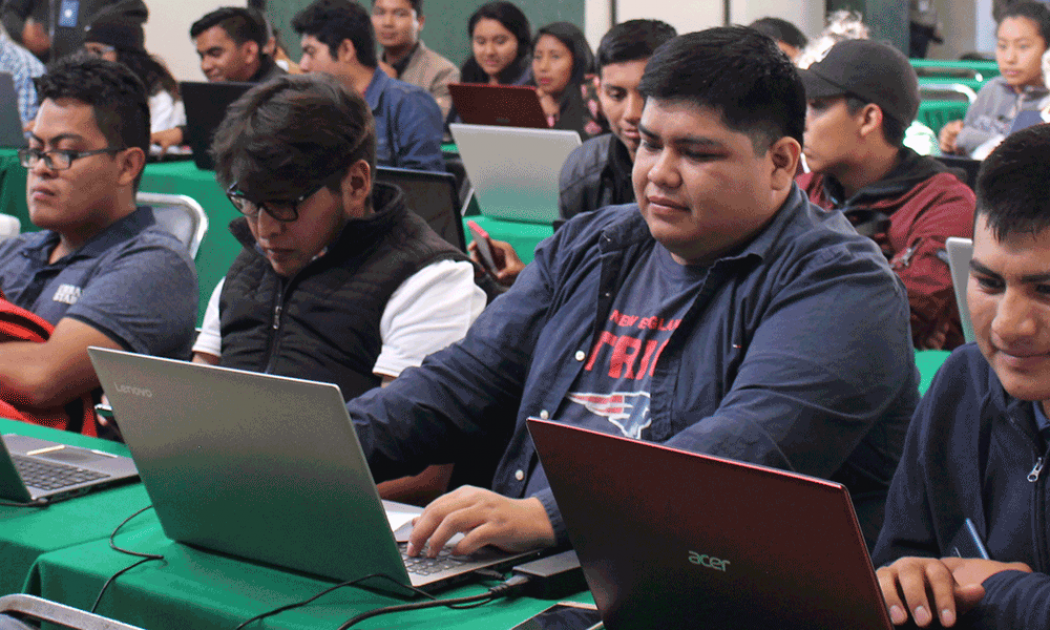
\includegraphics[width=\textwidth]{assets/est.png} % Imagen representativa

\column{0.65\textwidth}
\begin{exampleblock}{Camilo Soza - 20 años}
\begin{itemize}
\item Carrera: Derecho
\item Motivación: Investigación penal
\item Frustración: 
\begin{itemize}
\item Falta de espacios
\item Colas en Servicio Estudiantil
\end{itemize}
\end{itemize}
\end{exampleblock}
\end{columns}

\begin{alertblock}{Necesidad clave}
Reservar salas remotamente sin desplazamientos
\end{alertblock}
\end{frame}

\begin{frame}{Próximos pasos}
\centering
\Large
\begin{enumerate}
\item Desarrollo de prototipo
\item Pruebas de usabilidad
\item Implementación piloto
\end{enumerate}

\vspace{1cm}
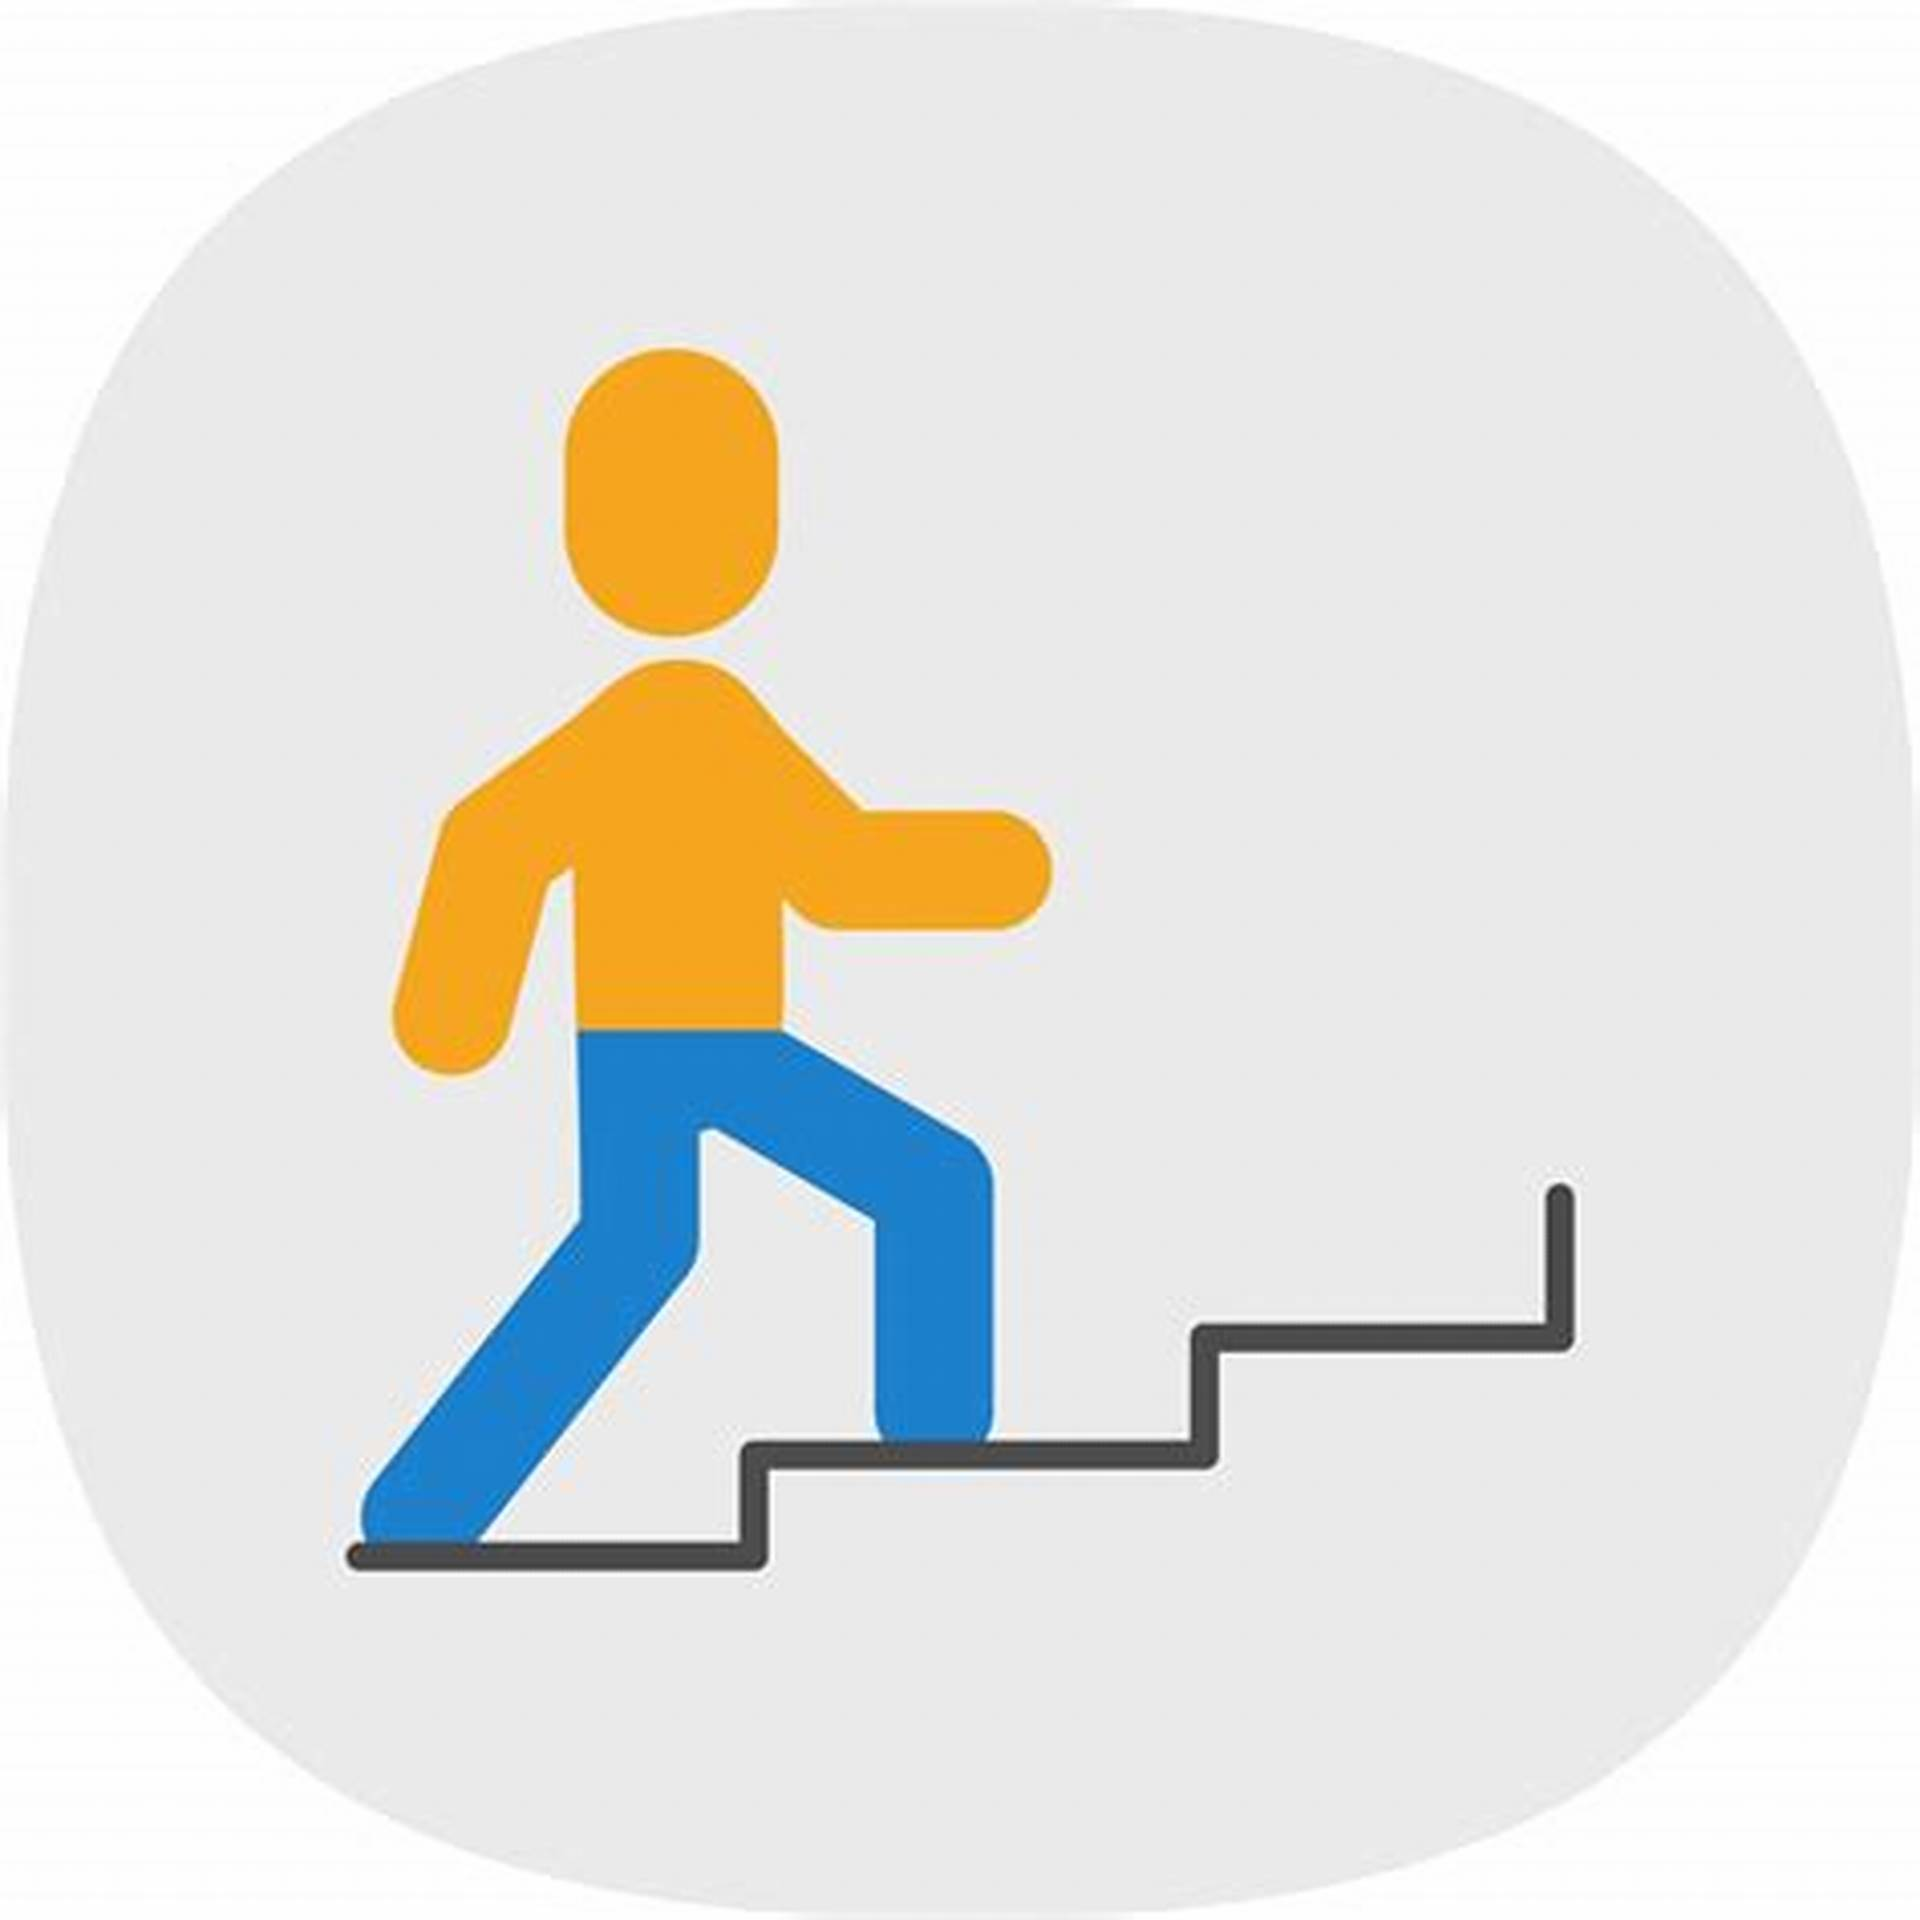
\includegraphics[height=1.5cm]{assets/next.jpeg} % Icono ilustrativo
\end{frame}

\end{document}